\documentclass[../main.tex]{subfiles}
\graphicspath{
    {"../img/"}
    {"img/"}
}

\begin{document}
    \subsection{Przygotowanie podłoża do tw (\ldots)}
    \subsubsection{Krzywizna}
    \begin{pytanie}
        Jak policzyć przyspieszenie dla nie-okręgów?
    \end{pytanie}
    \textbf{Odpowiedź: }A jaki jest promień tego aktualnego kółka?
    \begin{figure}[h]
        \centering
        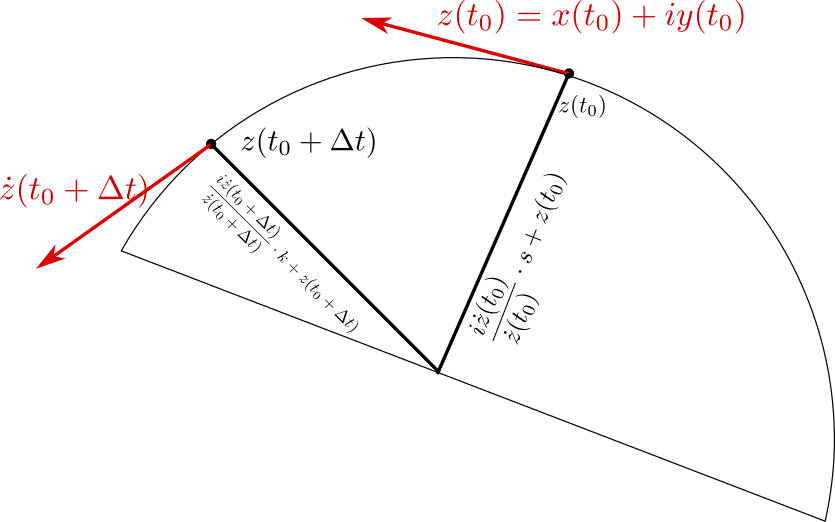
\includegraphics[width=0.6\textwidth]{w18-1}
        \caption{Liczymy na chama promień krzywizny}
        \label{fig:w18-1}
    \end{figure}
        Mamy jakąś krzywą (rys \ref{fig:w18-1})
        \[
            z(t) = x(t) + iy(t)
        .\]
    Szukamy tego punktu przecięcia z (rys \ref{fig:w18-1}): $\dot{z}(t) = \dot{x}(t) + i y(t)$, $z(t) = x(t) + iy(t)$
     \[
         \frac{i\dot{z}(t_0 + \Delta t)}{\left|z(t_0 + \Delta t)\right|} \cdot k + z(t_0 + \Delta t) = \frac{i\dot{z}(t_0)}{\left|\dot{z}(t_0)\right|}\cdot s + z(t_0)
    .\]
\begin{enumerate}[i)]
    \item Część urojona (wyrażamy $k$ przez $s$)
\[
    \frac{\dot{x}(t_0 + \Delta t)}{\left| \dot{z}(t_0 + \Delta t) \right| }\cdot k + y(t_0 + \Delta t) = \frac{\dot{x}(t_0)}{\left| \dot{z}(t_0) \right| }\cdot s + y(t_0)
.\]
Wyliczamy z tego $k$:
\[
    k = \frac{\left| \dot{z}(t_0 + \Delta t) \right| }{\dot{x}(t_0 + \Delta t)} \cdot  \frac{\dot{x}(t_0)}{|\dot{z}(t_0)|}\cdot s + \frac{\left| \dot{z}(t_0 + \Delta t) \right| }{\dot{x}(t_0 + \Delta t)}\cdot (y(t_0) - y(t_0 + \Delta t))
.\]
\item Część rzeczywista
    \[
        \frac{-\dot{y}(t_0 + \Delta t)}{\left| \dot{z}(t_0 + \Delta t) \right| }\cdot k + x(t_0 + \Delta t) = \frac{-\dot{y}(t_0)}{\left| \dot{z}(t_0) \right| }\cdot s + x(t_0)
    .\]
\[
    \frac{-\dot{y}(t_0 + \Delta t)}{\left| \dot{z}(t_0 + \Delta t) \right| }\cdot \frac{\left|\dot{z}(t_0 + \Delta t)\right|}{\dot{x}(t_0 + \Delta t)}\cdot \left( y(t_0) - y(t_0 + \Delta t) + x(t_0 + \Delta t) - x(t_0) \right) =
.\]
\[
    = s\cdot \left( \frac{-\dot{y}(t_0)}{\left| \dot{z}(t_0) \right| } + \frac{\dot{y}(t_0 + \Delta t)}{\dot{z}(t_0 + \Delta t)}\cdot \frac{\left| \dot{z}(t_0 + \Delta t)\right|}{\dot{x}(t_0 + \Delta t)}\cdot \frac{\dot{x}(t_0)}{\left| \dot{z}(t_0) \right| }  \right)
.\]
\item Mnożymy wszystko przez $\dot{x}(t_0 + \Delta t)$
\[
    -\dot{y}(t_0 + \Delta t)\left( y(t_0) - y(t_0 + \Delta t)\right) + \left(x(t_0 + \Delta t) - x(t_0)\right)\dot{x}(t_0 + \Delta t) =
\]
    \[
           = \frac{s}{\left| \dot{z}(t_0) \right| }\left( -\dot{y}(t_0)(\dot{x}(t_0 + \Delta t) + \dot{y}(t_0 + \Delta t) \cdot x(t_0)\right)
.\]
\item Dalej
    \[
        \dot{y}(t_0 + \Delta t)\left( y(t_0 + \Delta t) - y(t_0) \right) + \dot{x}(t_0 + \Delta t) (x(t_0 + \Delta t) - x(t_0)) =
    \]
    \[
        = \frac{s}{\left| \dot{z}(t) \right| }\left( \dot{x}(t_0)\left[ \dot{y}(t_0 + \Delta t) - \dot{y}(t_0) \right] - \dot{y}(t_0) \left[ \dot{x}(t_0 + \Delta t) - \dot{x}(t_0) \right]  \right)
    .\]
\item dzielimy wszystko przez $\Delta t$ i bierzemy granicę $\Delta t \to 0$
    \[
        \dot{y}(t_0) \cdot \dot{y}(t_0) + \dot{x}(t_0) \cdot \dot{x}(t_0) = \frac{s}{\left( \left( \dot{x}(t_0) \right) ^2 + \left( \dot{y}(t_0) \right) ^2 \right)^{\frac{1}{2}}} \left( \dot{x}(t_0) \cdot \ddot{y}(t_0) - \dot{y}(t_0) \cdot \ddot{x}(t_0) \right)
    .\]
    \item Zatem dostajemy wzór na krzywiznę $s$:
        \[
            \frac{1}{s} = \frac{\dot{x}\ddot{y} - \dot{y}\ddot{x}}{\left( \left( \dot{x} \right) ^2 + \left( \dot{y} \right)^2  \right)^{\frac{3}{2}} }
        .\]
\end{enumerate}
        \subsubsection{Inna fajna forma}
        Zauważmy, że $\bar{\dot{z}}(t) \cdot \ddot{z}(t) = \left( \dot{x}(t) - i\dot{y}(t) \right) + \left( \ddot{x}(t) + i\ddot{y}(t) \right) = \ldots + i\left( \dot{x}\ddot{y} - \dot{y}\ddot{x}(t) \right),$ czyli mając $z(t)$, policzymy krzywiznę tak:
        \[
            \frac{1}{s} = \frac{Im(\bar{\dot{z}}\ddot{z})}{\left| \dot{z} \right| ^3}
        .\]
    \begin{przyklad}
        Krzywa: $z(t) = 2e^{it}$, $\dot{z}(t) = 2ie^{it} = 2e^{i(t+\frac{\pi}{2})} \implies \bar{\dot{z}}(t) = 2e^{-i(t + \frac{\pi}{2})}$, $\ddot{z}(t) = -2e^{it}$.
        \[
            \bar{\dot{z}}\ddot{z} = -4 e^{i(t-t-\frac{\pi}{2})} = -4 \cdot (-i)
        .\]
    \[
        \frac{1}{s} = \frac{Im(4i)}{8} = \frac{4}{8} = \frac{1}{2}
    .\]
Czyli okrąg o promieniu $2$ ma promień równy $2$.
    \end{przyklad}
    \subsubsection{Odwzorowania konforemne}
    \begin{definicja}
        Niech $\Omega \subset\mathbb{R}^N$, $\Omega$ - spójny, $F$ - różniczkowalna na $\Omega$. Mówimy, że
        \[
        F : \Omega \to \mathbb{R}^N
        .\]
    jest odwzorowaniem konforemnym, jeżeli $F'$ jest proporcjonalna do macierzy ortogonalnej.
    \[
        F'(x) = f(x) \cdot R(x)
    ,\]
gdzie $f(x) : \Omega \to R$, a $R(x)$ - macierz  $n\times n$ taka, że
 \[
     R(x)^{-1} = \left( \bar{R}(x) \right) ^T,\quad \det R(x) = 1
.\]
    \end{definicja}
    \begin{stw}
        (\textbf{Wniosek:}) odwzorowanie konforemne zachowuje kąt między stycznymi do krzywych.
    \end{stw}
    \begin{proof}
Weźmy dwie krzywe sparametryzowane
\[
    x_1(t),\quad t\in ]-a,a[
\]
\[
    x_2(t),\quad t\in ]-b,b[
\]
        i
        \[
            x_1(0) = x_1(0).
        \]
        Wówczas ($\gamma$ - kąt między krzywymi)
        \[
            \cos\gamma = \frac{\left<\dot{x}_1 | \dot{x}_2 \right>_{t=0}}{\left\Vert \dot{x}_1 \right\Vert \left\Vert \dot{x}_2 \right\Vert _{t=0}}
        .\]
    Policzmy kąt między stycznymi do krzywych $F(x_1(t)), F(x_2(t))$
    \[
        \cos\gamma' = \frac{\left<\frac{d}{dt}F(x_1(t))_{t=0} | \frac{d}{dt}F(x_2(t))_{t=0} \right>}{\left\Vert \ldots \right\Vert \left\Vert \ldots \right\Vert }
    ,\]
ale my wiemy, że
 \[
     \frac{d}{dt}F(x_1(t))_{t=0} = F'(x_1(t)) \frac{d}{dt}x_1(t)_{t=0}=
\]
F - konforemna, więc
\[
    = f(x_1(t))R(x_1(t))\dot{x}_1(t)_{t=0}
.\]
Pamiętamy, że jeżeli $R$ - ortogonalna, to $\left<x|y \right> = \left<Rx|Ry \right>$, zatem
\[
    \cos\gamma' = \frac{\left<f\cdot R\dot{x}_1 | f\cdot R\dot{x}_2 \right>_{t=0}}{\left\Vert f\cdot R\dot{x}_1 \right\Vert \left\Vert f\cdot R \dot{x}_2 \right\Vert_{t=0} } =
        \frac{\left<\dot{x}_1 | \dot{x}_2 \right>}{\left\Vert \dot{x}_1 \right\Vert \left\Vert \dot{x}_2 \right\Vert _{t=0}} = \cos\gamma
.\]
    \end{proof}
    \begin{pytanie}
        A co z funkcjami zespolonymi?
    \end{pytanie}
    \textbf{Odpowiedź: }Niech
    \[
        f(z) = f(x + iy) = f_1(x,y) + if_2(x,y)
    ,\]
taka, że $f$ - holomorficzna. Możemy zatem badać funkcję
\[
    F(x,y) = \begin{bmatrix} f_1(x,y)\\ f_2(x,y) \end{bmatrix}
.\]
Wówczas
\[
    F'(x,y) = \begin{bmatrix} \frac{\partial f_1}{\partial x} & \frac{\partial f_1}{\partial y} \\ \frac{\partial f}{\partial x} & \frac{\partial f_2}{\partial y}  \end{bmatrix} \overset{\text{C-R}}{=} \begin{bmatrix} \frac{\partial f_1}{\partial x} &-\frac{\partial f_2}{\partial x} \\\frac{\partial f_2}{\partial x} &\frac{\partial f_1}{\partial x}  \end{bmatrix} = \begin{bmatrix} a&-b\\b&a \end{bmatrix}
.\]
Jeżeli $R = \begin{bmatrix} a&b\\c&d \end{bmatrix} $ i $R$ - ortogonalna, to znaczy, że $R^{-1} = \bar{R}^{T}$ i $\det R = 1$
     \[
         \frac{1}{ad - bc}\begin{bmatrix} d&-b\\ -c&a \end{bmatrix} = \begin{bmatrix} a&c\\b&d \end{bmatrix} \implies d = a \land -b = c
    .\]
Czyli
\[
    F'(x,y) = (a^2 + b^2)\frac{1}{a\cdot a - (-b)\cdot b}\begin{bmatrix} a&-b\\b&a \end{bmatrix}
.\]
\subsection{Powrót do residuów w nieskończoności}
mamy
\[
    g(z) = f\left(\frac{1}{z}\right) = \sum_{n=-\infty}^{\infty} a_n z^n,\quad z\in R(0,0,r)
.\]
Oznacza to, że
\[
    f(z) = g\left( \frac{1}{z} \right) = \sum_{n=-\infty}^{\infty} a_n \frac{1}{z^n},\quad |z| > \frac{1}{r}
.\]
Zauważmy, że $a_n$ w rozwinięciu $g(z)\ldots$ jest dany wzorem
\[
    a_n = \frac{1}{2\pi i} \int\limits_{\substack{\partial K(0,t)\\ 0 < t < r}} \frac{g(z)}{z^{n+1}}dz
.\]
Zamieniamy zmienne: $z = \frac{1}{z'}$, $dz = -\frac{1}{(z')^2}$
 \[
     a_n = \frac{1}{2\pi i} \int\limits_{\substack{\partial K\left(0,\frac{1}{t}\right)\\ 0 < t < r}} \frac{g\left( \frac{1}{z'} \right) }{\left( \frac{1}{z'} \right) ^{n+1}}\cdot \frac{-1}{(z')^2}dz' = \int\limits_{\substack{\partial K(0,\frac{1}{t}\\ 0 < t < r}}f(z')(z')^{n-1}dz'
 .\]

\end{document}
